\documentclass[conference,compsoc,a4paper,twocolumn,final]{IEEEtran}

\usepackage[utf8]{inputenc}
\usepackage[T1]{fontenc}
\usepackage{lmodern}
\usepackage{couriers}

\ifCLASSOPTIONcompsoc
  % IEEE Computer Society needs nocompress option
  % requires cite.sty v4.0 or later (November 2003)
  \usepackage[nocompress]{cite}
\else
  % normal IEEE
  \usepackage{cite}
\fi

\ifCLASSINFOpdf
  \usepackage[pdftex]{graphicx}
  % declare the path(s) where your graphic files are
  \graphicspath{../images/}
  % and their extensions so you won't have to specify these with
  % every instance of \includegraphics
  \DeclareGraphicsExtensions{.jpg,.png}
\else
  % or other class option (dvipsone, dvipdf, if not using dvips). graphicx
  % will default to the driver specified in the system graphics.cfg if no
  % driver is specified.
  % \usepackage[dvips]{graphicx}
  % declare the path(s) where your graphic files are
  % \graphicspath{{../eps/}}
  % and their extensions so you won't have to specify these with
  % every instance of \includegraphics
  % \DeclareGraphicsExtensions{.eps}
\fi

%% Package for non-breaking URL.
\usepackage{url}

%% \multirow{package}{width}{text}
\usepackage{multirow}

%% Package for reading CSV to database.
\usepackage{datatool}

%% Tikz
\usepackage{tikz}
\usetikzlibrary{backgrounds, shapes.geometric, positioning, patterns, external}
	\tikzexternalize

%% Make tikz generate PDF file to .tmp directory
\makeatletter
	\newcommand{\mytikzinput}[1]{%
		\tikzsetnextfilename{tmp/#1}%
	}
\makeatother

%% Pgfplots
\usepackage{pgfplots}

%% MnSymbol
\usepackage{MnSymbol}

%% Set spacing on table.
\renewcommand{\arraystretch}{1.5}
\setlength{\tabcolsep}{3pt}

%%% uncomment this to show overrule in black box
\overfullrule=2cm

\hyphenation{
	Be-ri-kut
	Ja-nu-a-ri
	SIGKDD
	Wiki-pedia
	a-kan
	a-ku-ra-si
	a-na-li-sis
	ang-ka
	ba-gai-ma-na
	bayes-ian
	ber-gu-na
	ber-kas
	ber-ma-sa-lah
	ber-mak-na
	bi-a-ya
	da-lam
	data-set
	de-ngan
	di-ha-sil-kan
	di-pi-lih
	di-sam-pel
	di-sing-kat
	di-tam-bah
	di-tam-bah-kan
	di-te-rap-kan
	dis-krit
	fung-si
	ga-bung-an
	ke-las
	ke-le-mah-an
	ke-mung-ki-nan
	ke-tak-se-imbang-an
	lan-guage
	ma-yo-ri-tas
	me-laku-kan
	me-me-rik-sa
	me-mi-lih
	me-ne-rap-kan
	meng-a-pli-ka-si-kan
	meng-ge-ne-ra-li-sa-si
	me-ning-kat-kan
	me-nye-dia-kan
	me-nye-im-bang-kan
	me-sin
	me-thod
	me-to-de
	mem-vi-sua-li-sa-si
	meng-gu-na-kan
	meng-hi-lang-kan
	meng-hu-bung-kan
	meng-i-kut-kan
	meng-i-kuti
	meng-im-ple-men-ta-si-kan
	meng-in-di-ka-si-kan
	me-re-pre-sen-ta-si-kan
	mi-sal-nya
	mung-kin
	o-pe-ra-si
	o-ver-sam-pling
	pa-ra-lel
	pe-la-ti-han
	pe-mi-sah
	pe-nan-da
	pe-ne-li-ti-an
	pe-ngu-ji-an
	pe-nu-li-san
	pe-nyun-ting
	pem-ban-ding
	pen-de-kat-an
	peng-kla-si-fi-ka-si
	peng-a-pli-ka-si-an
	per-for-man-si-nya
	po-ten-si-al
	pro-ba-bi-li-tas
	pro-per-ti
	pro-ses
	sam-pel
	se-im-bang
	se-jum-lah
	sun-ting-an
	ting-kat
	un-der-sam-pling
	wa-lau-pun
}

\newcommand{\judul}{%
	Deteksi Vandalisme pada Wikipedia Bahasa Inggris Menggunakan
	Sampel Ulang LNSMOTE
	dan Klasifikasi Cascaded Random Forest
}
\newcommand{\mytitle}{%
	Detecting Vandalism on English Wikipedia using LNSMOTE Resampling and
	Cascaded Random Forest Classifier
}
\newcommand{\myname}{Muhamad Sulhan}
\newcommand{\mysid}{23513014}
\newcommand{\myemail}{ms@students.itb.ac.id}
\newcommand{\myschool}{School of Electrical and Informatics Engineering}
\newcommand{\tfakultas}{Sekolah Teknik Elektro dan Informatika}

\newcommand{\myadvisorname}{Dwi Hendratmo Widyantoro}
\newcommand{\myadvisorshortname}{Dwi H. Widyantoro}
\newcommand{\myadvisorid}{196812071994021001}
\newcommand{\myadvisoremail}{dwi@stei.itb.ac.id}
\newcommand{\mydept}{Program Studi Magister Informatika}

\newcommand{\itb}{Institut Teknologi Bandung}
\newcommand{\itbaddress}{Ganesha 10, Bandung, Indonesia 40132}

\newcommand{\tUpAbstrak}{ABSTRAK}
\newcommand{\tupabstract}{ABSTRACT}
\newcommand{\tuppengesahan}{HALAMAN PENGESAHAN}

\newcommand{\daftarisi}{DAFTAR ISI}
\newcommand{\tupdaftarlampiran}{DAFTAR LAMPIRAN}
\newcommand{\daftargambar}{DAFTAR GAMBAR DAN ILUSTRASI}
\newcommand{\daftartabel}{DAFTAR TABEL}

\newcommand{\tDaftarPustaka}{DAFTAR PUSTAKA}
\newcommand{\tLampiran}{Lampiran}
\newcommand{\tUpLampiran}{\MakeUppercase{\tLampiran}}

%%% My images directory
\graphicspath{{../images/} {images/}}
\newcommand{\myitbcover}{ITB-logo-hitam}
\newcommand{\myitbcoverblue}{ITB-logo-ganesha}



\begin{document}

\IEEEoverridecommandlockouts
\IEEEpubid{%
	\makebox[\columnwidth]{%
\hfill%
978-1-5090-1636-5/16/\$31.00~\copyright2016 IEEE%
\hfill%
	}
	\makebox[\columnwidth]{}
}

\title{\mytitle}

\author{
	\IEEEauthorblockN{
		\myname\IEEEauthorrefmark{1}
		and
		\myadvisorshortname\IEEEauthorrefmark{2}
	}
	\IEEEauthorblockA{
		\myschool\\
		\itb\\
		\itbaddress\\
		Email:
		\IEEEauthorrefmark{1}ms@students.itb.ac.id,
		\IEEEauthorrefmark{2}dwi@stei.itb.ac.id
	}
}

\maketitle


\begin{center}
\textbf{\large
	\MakeUppercase{\mytitle{}} \\
	\bigskip
	\textnormal{By} \\
	\myname{} \\
	NIM: \mysid{} \\
	(\mydept{}) \\
}
\end{center}

\bigskip
\bigskip
\bigskip

Wikipedia.org is an online encyclopedia which can edited by anyone.
Those feature has benefit, which make the article in Wikipedia rapidly
increased in size and can be fixed subsequently, and their drawbacks was prone
to vandalism in the forms of invalid information, deletion, ads, or meaningless
content.
This paper propose a framework for detecting vandalism on English Wikipedia
using machine learning technique by training Cascaded Random Forest (CRF)
classifier on English Wikipedia dataset (PAN-WVC-10) that has been resampled
using Local Neighbourhood SMOTE (LNSMOTE).
Those two methods then compared with Random Forest (RF) for classifier and
SMOTE for resampling.
The result of training both classifiers that has been tested on Wikipedia
Vandalism Corpus 2011 (PAN-WVC-11) English only dataset showed that the dataset
resampled using LNSMOTE have true-positive rate better than SMOTE.
CRF on LNSMOTE with 200 stages and 1 tree gave the better result among others
with TPR value 0.9904.
From training computation time, CRF 1.6 times faster than RF in resampled
dataset.

Keywords: wikipedia, vandalism, imbalanced dataset, dataset resampling,
cascaded random forest


\section{Introduction}
\label{section:introduction}
	Vandalism, according to Merriam-Webster's dictionary is willful or malicious
destruction or defacement of public or private property.
In the context of Wikipedia, vandalism can be in the form of malicious edit
which intends to give wrong information, hiding information by deleting
the content, abusive content, ads, and/or meaningless text.
Finding and fixing the article that has been vandalized can disrupt the editor
from writing or expanding new article or other important tasks, and for the
reader they will get the wrong information or no information at all due to
deletion.

Corpus that commonly used for learning vandalism on Wikipedia is PAN Wikipedia
Vandalism Corpus 2010 (PAN-WVC-10)
\cite{potthast:2010b}
or PAN Wikipedia Vandalism Corpus 2011 (PAN-WVC-11)
\cite{potthast:2010b}.
Both of the corpus have class imbalance problem.
PAN-WVC-10 for an English articles have 32,439 sample with only $2,394$ (7.38\%)
of them is vandalism, whereas PAN-WVC-11 for an English articles have $9,985$
sample with only $1,144$ (11.45\%) of them are vandalism.

Training a classifier on imbalance dataset could lead to low performance.
This can be caused either by the minority class has low contribution to error
rate, which makes the classifier bias to majority class, or some classifier
assume that class distribution is balanced, while in real world cases this
rarely happened.

Random Forest (RF) has the disadvantages in their computation time
especially when training the classification model.  For a large dataset with
more than 10,000 samples (like the PAN-WVC-10 cases) this could lead to hours
of training time.  One of the solution is by using Cascaded Random Forest (CRF)
framework proposed by Bauman et al. \cite{baumann2013cascaded}.
Their paper state that CRF give a fast training model time and increased
performance compared to RF.

This paper attempts to overcome the dataset imbalance problem on PAN-WVC-10 by
applying resample and classifier technique that has never been used before on
the dataset.
The PAN-WVC-10 dataset is resampled using Local Neighborhood SMOTE (LNSMOTE)
technique,
which proposed by Maciejewski and Stefanowski
\cite{maciejewski2011local}.
The result from resampling then trained using CRF classifier and compared with
RF classifier to see their performance.

This paper is organized as follow.
Section \ref{section:related_works} briefly review past researches on vandalism
detection on Wikipedia.
Section \ref{section:literature_study} review the LNSMOTE and CRF techniques.
Section \ref{section:research_methodology} describes the process to generate
features from raw dataset and resampling process before it was trained and
tested on classifiers.
Section \ref{section:result_and_analysis} shows the result from each classifier
on each dataset and their analysis.
Section \ref{section:conclusion} concludes the experiments and
give some possible future works that can be extended from this paper.

\IEEEpubidadjcol


\section{Related Works}
	\label{section:related_works}
	Vandalism detection in Wikipedia based on machine learning approach
became an interesting research topic since 2008.
Potthast et al. \cite{potthast2008automatic} contribution is the first vandalism
detection approach using machine learning with textual and basic
metadata features using Logistic Regression classifier.
Smets et al. \cite{smets08automaticvandalism} use Naive Bayes classifier on
selected words that representing vandalism edit and the first who use
compression model to detect vandalism in Wikipedia.
Itakura and Clarke \cite{itakura2009using} use Dynamic Markov Compression to
detect vandalism edit in Wikipedia.
Mola Velasco \cite{mola2012wikipedia} extend the Potthast research by adding
more textual features and word-list features.
West and Lee \cite{west2011multilingual} use spatial and temporal metadata
without required to check the text in the article and revision, and the first
to introduce \textit{ex post facto} data as feature, where prediction
take the next revision into consideration.
Adler et al. \cite{adler2011wikipedia} build a vandalism detection system using
reputation called WikiTrust and then combine it with
natural language, spatial and temporal features.
Harpalani et al. \cite{harpalani2011language} propose that vandalism has
a unique and equal lingustic property.
They build a system for detecting vandalism based on \textit{stylometric}
analysis from vandalism edit with \textit{context-free grammar} probabilistic
model.
Following the trend of classifying on cross-language vandalism, Tran and
Christen \cite{tran2013cross} evaluated several classifier based on
language feature collected from number of article viewed every hours and the
history of their edit in Wikipedia.

Gotze \cite{gotze2014advanced} combine features from
\cite{potthast2008automatic},
\cite{mola2012wikipedia},
\cite{west2011multilingual},
\cite{adler2011wikipedia},
\cite{javanmardi2011vandalism},
and
\cite{wang2010got},
with four additional and modified features.
Gotze use the random oversampling technique, to overcome imbalance problem,
called
\textit{Synthetic Minority Over-sampling TEchnique} (SMOTE)
proposed by Chawla et al.
\cite{chawla2002smote}.
Original and resampled dataset of PAN-WVC-10 then tested with two-class
classifier:
\textit{Logistic Regression},
\textit{RealAdaBoost},
\textit{Random Forest} (RF), and
\textit{Bayesian Network}.
His evaluation on original dataset showed that RF give better result than
others classifiers.
The result from resampling dataset showed increasing in performance on all
classifiers except RF.

From the previous research, seven of them
(
\cite{mola2012wikipedia}
\cite{west2011multilingual}
\cite{adler2011wikipedia}
\cite{harpalani2011language}
\cite{gotze2014advanced}
\cite{wang2010got}
\cite{adler2010detecting}
)
use PAN-WVC-10,
with the best precision value is $0.86$ and recall value is $0.57$, which
obtained by Velasco using RF without resampling on dataset.
Only two research
(
\cite{west2011multilingual}
\cite{gotze2014advanced}
)
that use PAN-WVC-11
with the best result obtained by Gotze, $0.92$ on precision and $0.39$
on recall.


\section{Literature Study}
	\label{section:literature_study}

This section review the techniques used for implementation in this paper.

\subsection{LNSMOTE}
	\label{subsection:lnsmote}
	Meskipun hasil SMOTE dibuktikan bagus dalam makalah Chawla dkk.
\cite{chawla2002smote}, metode ini masih memiliki beberapa kelemahan.
Pertama, cara menentukan sampel minoritas sebagai calon untuk
\textit{over-sampling} bisa bermasalah.
Pada SMOTE, semua sampel dari kelas minoritas digunakan.
Namun, bukan berarti semua sampel tersebut sama bergunanya bagi pembelajaran
klasifikasi.
Pada khususnya, sampel yang ada pada batas \textit{decision}, atau berada
dibatas kelas minoritas dengan kelas mayoritas, lebih sering salah
diklasifikasi dibandingkan dengan sampel yang berada jauh dari batas kelas,
oleh karena itu mereka lebih penting untuk klasifikasi.
Sampel yang jauh dari batas kelas, berada di tengah kelas minoritas mungkin
berkontribusi sedikit pada klasifikasi.
Salah satu metode untuk menangani permasalahan ini yaitu dengan hanya
mengambil sampel pada batas kelas minoritas yang dijadikan untuk
\textit{oversampling}, seperti yang diajukan oleh Han dkk.
\cite{han2005borderline} dengan menggunakan metode bernama \textit{Borderline
SMOTE}.

\begin{figure}[htbp]
	\centering
	\begin{subfigure}[b]{0.4\textwidth}
		\centering
		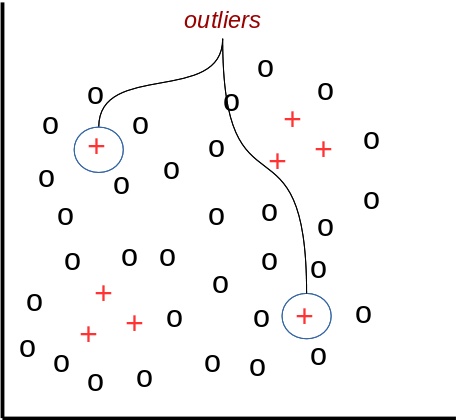
\includegraphics[width=\textwidth]{SMOTE-problem-outliers}
		\caption{}
		\label{fig:smote-outliers}
	\end{subfigure}
	\begin{subfigure}[b]{0.5\textwidth}
		\centering
		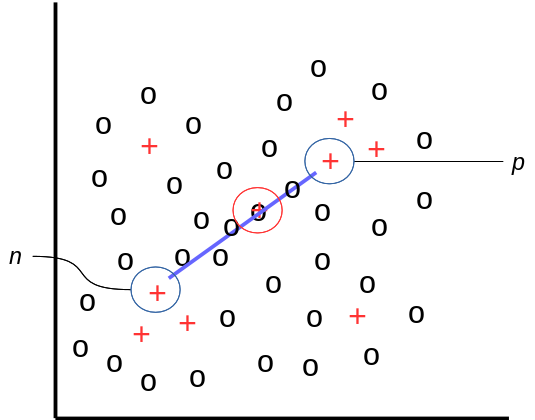
\includegraphics[width=\textwidth]{SMOTE-problem-overlapping}
		\caption{}
		\label{fig:smote-overlapping}
	\end{subfigure}
	\caption{
Kelemahan metode SMOTE:
(a) \textit{Outliers} pada kelas minoritas tidak diperhitungkan pada metode
SMOTE.
(b) Pembuatan sampel sintetis yang baru berada di wilayah kelas mayoritas
yang tumpang-tindih dengan sampel kelas mayoritas.
	}
	\label{fig:smote-problems}
\end{figure}

Kelemahan lain dari SMOTE yaitu permasalahan \textit{overgeneralization} yang
begitu saja menggeneralisasi wilayah dari kelas minoritas.
SMOTE tidak mempertimbangkan distribusi dari sampel pada kelas mayoritas, atau
adanya \textit{outliers}.

Untuk mengatasi permasalahan di atas, Maciejewski dkk. memperkenalkan ekstensi
dari metode SMOTE bernama \textit{Local-neighbourhood SMOTE} atau disingkat
LNSMOTE \cite{maciejewski2011local} yang menggunakan modifikasi dari
pendekatan \textit{Safe-Level SMOTE} \cite{bunkhumpornpat2009safe}.
Pada metode \textit{Safe-level SMOTE} keberadaan sampel mayoritas
diperhitungkan sebelum membuat sampel sintetis dengan menghitung sebuah
koefisien khusus yang disebut \textit{safe level}.
Untuk setiap sampel dari kelas minoritas, dihitung jumlah sampel kelas
minoritas di antara \textit{k-nearest-neighbors} (KNN).
Jika nilainya sama atau mendekati $ 0 $, sampel tersebut dianggap sebagai
\textit{noise}.
Jika nilainya mendekati $ k $, maka sampel tersebut bisa dikatakan berada
di wilayah aman dari kelas minoritas.
Gagasan utamanya adalah membuat sampel sintetis yang dekat dengan wilayah aman.

Lebih rincinya, misalkan $ p $ adalah sampel dari kelas minoritas yang akan
menjadi calon untuk \textit{over-sampling}, maka $ k $ sampel terdekat dengan
$ p $ yang termasuk pada kelas minoritas $ P $ ditentukan.
Seperti pada SMOTE, setidaknya satu dari tetangga tersebut dipilih, sebutlah
dengan $ n $.
Untuk kedua sampel, $ p $ dan $ n $, $ k $ sampel terdekatnya untuk keseluruhan
data pelatihan $ S $ dihitung \textit{safe level}-nya dengan notasi $ sl(p) $
dan $ sl(n) $.
Dari pengetahuan tersebut, koefisien rasio \textit{safe-level} ditentukan
dengan $ \textit{sl-ratio} = sl(p) / sl(n) $.
Langkah selanjutnya ditentukan berdasarkan 5 kasus berikut:
\begin{enumerate}
	\item \label{case:safe-1} Jika $ sl(p) = 0 $ dan $ sl(n) = 0 $, sampel
	$ p $ dan $ n $ dianggap sebagai \textit{noise outliers}, dan tidak ada
	sampel sintetis yang dibuat.
	\item Jika $ sl(p) > 0 $ dan $ sl(n) = 0 $, maka $ n $
	adalah \textit{noise}.
	Sampel sintetis akan dibuat jauh dari $ n $ dengan menduplikasi $ p $.
	\item Jika $ sl-ratio = 1 $, maka $ p $ dan $ n $ memiliki tetangga
	yang sama dan sampel sintetis yang baru akan dibuat diantara garis yang
	menghubungkan mereka dengan cara yang sama seperti pada SMOTE.
	\item Jika $ sl-ratio > 1 $, maka $ p $ berada di wilayah
	aman minoritas daripada $ n $ dan sampel sintetis yang baru akan
	dibuat dekat dengan $ p $, dengan parameter acak pada SMOTE akan
	memiliki rentang $ [0, 1 / \textit{sl-ratio}] $.
	\item Jika \textit{sl-ratio < 1}, maka \textit{n} berada di wilayah
	aman minoritas daripada $ p $ dan sampel sintetis yang baru akan
	dibuat dekat dengan $ n $, yaitu parameter acak pada SMOTE akan
	memiliki rentang $ [1 - \textit{sl-ratio}, 1] $.
\end{enumerate}

Strategi \textit{safe-level SMOTE} bermasalah khususnya pada distribusi kelas
yang bias yang mana kelas minoritas menyebar sehingga terdiri dari beberapa
sub-wilayah dengan kardinalitas yang kecil.
Situasi ini mengacu pada permasalahan yang disebut \textit{small disjuncts}
yang diakui sebagai sumber kesulitan yang paling penting bagi pembelajaran
klasifikasi untuk data timpang \cite{jo2004class}.
Pada kasus seperti ini pembuatan sampel sintetis dengan \textit{Safe-level
SMOTE} bisa menyebabkan terjadinya tumpang-tindih antara kelas.

Sebagai contohnya, misalkan dua kelompok dari kelas minoritas terpisah
dikelilingi oleh sampel dari kelas mayoritas.
Katakanlah, jarak antara kedua kelompok minoritas tersebut cukup jauh, satu
kelompok berada di bawah dan kelompok lainnya di atas.
Misalkan calon dari sebuah sampel berada di kelompok yang dibawah.
Jika parameter $ k $ dari fungsi pencarian KNN lebih besar dari jumlah sampel
kelas minoritas di dalam kelompok tersebut, maka tetangga dari kelas minoritas
selanjutnya akan menjadi sampel dari kelompok yang lain.
Jika rasio \textit{safe-level} dari sampel kedua kelompok sama, sampel sintetis
yang baru bisa dibuat diantara garis yang menggabungkan sampel-sampel dari
kedua kelompok tersebut.
Dengan kata lain, sampel sintetis yang baru bisa berada di wilayah yang dihuni
oleh kelas mayoritas.
Makanya, strategi ini masih memungkinkan terjadinya tumpang-tindih antara
kelas.

Situasi tidak diinginkan seperti di atas disebabkan karena teknik SMOTE mencari
KNN yang dimiliki oleh kelas minoritas saja.
Jika calon sampel tidak berada di wilayah yang padat dengan kelas minoritas,
maka beberapa tetangganya bisa saja cukup jauh dan juga sampel dari kelas
mayoritas mengelilingi calon sampel tersebut.

LNSMOTE mengatasi masalah tumpang tindih ini dengan lebih mempertimbangkan
tetangga sekitar
(\textit{local neighbourhood})
dari calon sampel minoritas yang mungkin bisa memberikan perkiraan dari
keberadaan sampel kelas mayoritas.
Jadi, pencarian sampel yang terlalu jauh sebaiknya dihindarkan.

Modifikasi teknik LNSMOTE terhadap \textit{Safe-Level} SMOTE yaitu,
\begin{itemize}
\item jika calon sampel $ p $ diidentifikasi berada di tetangga terdekat $ k
$ dari $ n $, sampel tersebut tidak langsung dihitung dengan $ sl(n) $ tapi
dicari tetangga dari $ k + 1 $ selanjutnya.
\item Membatasi rentang interval di mana sampel baru secara acak ditempatkan.
Jadi, pada beberapa kasus dari \textit{safe-level}, LNSMOTE tidak menentukan
batas kanan dari interval dengan 1 tapi sebagai ambang batas $\tau < 1$.
Ambang batas tersebut tidak baku tapi ditentukan secara dinamis bergantung
kepada \textit{safe-level} dari sampel mayoritas.
\item Jika $ sl(n) $ relatif rendah, artinya $ n $ dikelilingi oleh banyak
sampel dari kelas mayoritas, sampel baru seharusnya ditempatkan lebih dekat ke
$ p $.
\item Jika $ n $ dikelilingi oleh sejumlah sampel minoritas yang seimbang,
sehingga nilai $ sl(n) $ tinggi, sampel yang baru bisa berada di dekat $ n $.
Hal ini supaya bisa mengontrol tingkat ekspansi dari kelas minoritas dengan
cara dinamis, memperhitungkan distribusi lokal dari sampel.
\end{itemize}

Algoritma LNSMOTE yang digunakan pada implementasi tesis berdasarkan pada
makalah Maciejewski dkk.
\cite{maciejewski2011local}
yang dapat dilihat pada lampiran
\ref{lampiran:alg_lnsmote}.


\subsection{Cascaded Random Forest}
	\label{subsection:crf}
	Permasalahan umum dalam penggalian data atau algoritma pembelajaran ansambel
adalah ketidakmampuan untuk menangani data pelatihan yang timpang.
Ketimpangan antara kelas positif dan negatif biasanya menyebabkan akurasi
deteksi yang rendah.
Simulasi yang dilakukan oleh Strobel dkk. \cite{strobl2007bias} menampilkan
bahwa RF condong mendukung kelas mayoritas.
Saat menggunakan RF untuk deteksi, sejumlah besar sampel negatif dibutuhkan
untuk mendapatkan pengklasifikasi yang kuat dan laju \textit{false-positive}
yang rendah.
Hal ini menyebabkan ketimpangan yang besar antara kelas positif dan
negatif, sehingga membuat pengklasifikasi RF yang berfokus pada kelas
mayoritas.
Kelemahan lain dari RF yaitu setelah belajar dengan beberapa pohon, RF secara
gradual mencapai titik puncaknya, yang mana pengklasifikasi tidak bisa lagi
meningkatkan \textit{sensitivity} pada pendeteksian maupun mengurangi laju
\textit{false-positive}-nya.

Pada tahun 2011, Viola dan Jones mengajukan algoritma deteksi sampel cepat
berbasis AdaBoost dengan struktur kaskade (\textit{cascade})
\cite{viola2004robust}.
Struktur kaskade dimotivasi oleh asumsi bahwa lebih mudah untuk menolak sebuah
sampel yang negatif daripada mencari sampel yang positif.
Viola dan Jones menggabungkan pengklasifikasi yang kuat pada beberapa tingkatan
yang independen dengan kondisi bahwa setiap tingkat dapat menolak sebuah
sampel, sehingga supaya sebuah sampel dapat dianggap positif semua tingkat
harus terlewati.
Disebabkan karena dominasi penolakan pada tahap-tahap awal, waktu komputasi
menjadi berkurang.
Sebagai tambahan, untuk mendapatkan pelatihan yang lebih baik, Viola dan Jones
mengajukan strategi \textit{bootstrap} dengan menghapus sampel yang benar
terklasifikasi negatif setelah pembelajaran dilakukan pada setiap tingkat.
Setelah itu, dataset pelatihan yang berkurang ditambahkan dengan sampel yang
salah diklasifikasi (\textit{false-positive})
\cite{viola2004robust}.

Sebuah pengklasifikasi kaskade terdiri dari sejumlah tingkatan dengan
kompleksitas yang meningkat.
Setiap tingkat minimum memiliki satu pengklasifikasi independen.
Pengklasifikasi ditambahkan ke dalam tingkatan sampai batas nilai
\textit{true-positive} dan \textit{true-negative} tercapai.
Keuntungan dari struktur kaskade yaitu sejumlah besar sampel dapat
didistribusikan diantara tingkatan, berkurangnya nilai \textit{false-positive},
dan berkurangnya waktu komputasi baik pada pelatihan dan klasifikasi.

Baumann menerapkan metoda ini pada RF dan mengajukan \textit{Cascaded Random
Forest} (CRF) yaitu penggabungan dari pengklasifikasi RF dengan struktur
kaskade, yang menyusun beberapa pohon keputusan dalam setiap tingkatan dengan
strategi agregasi \textit{bootstrap}.
Sehingga, pembelajaran pada sampel positif meningkat dan kelemahan dari data
yang timpang terhindari \cite{baumann2013cascaded}.

Pengklasifikasi CRF memiliki enam parameter umum, tiga diantaranya sama dengan
RF yaitu jumlah pohon ($T$), persentase sampel acak untuk \textit{bootstrap},
($b$), dan jumlah fitur acak ($m$).
Tiga parameter lainnya yaitu jumlah tingkatan ($S$), nilai ambang batas
\textit{true-positive} ($maxtp$), dan nilai ambang batas
\textit{true-negative} ($maxtn$).

Strategi \textit{bootstrap} yang digunakan adalah sebagai berikut: setelah
menyelesaikan pembelajaran pada sebuah tingkatan, dataset pelatihan yang berisi
hanya sampel negatif diujikan ke semua tingkatan yang telah dibentuk
sebelumnya dengan tujuan untuk menghapus sampel yang benar bernilai
\textit{true-negative} saja, sehingga dataset pelatihan sebisa mungkin berisi
hanya sampel positif.
Sampel yang terklasifikasi \textit{false-positive} kemudian dimasukan kembali
ke dataset pelatihan untuk dipelajari oleh tingkatan berikutnya.
Fungsi selengkapnya dari CRF dapat dilihat pada algoritma \ref{alg:crf}.

Beberapa tingkatan memiliki akurasi deteksi yang lebih rendah daripada
yang lainnya.
Untuk mengurangi pengaruh tingkatan yang memiliki performansi yang rendah
tersebut, maka dihitung faktor bobot $\alpha$ dari setiap tingkatan dengan
mengeksploitasi rerata harmonik dari \textit{precision} dan \textit{recall},
atau dikenal juga dengan nilai $F_1$ (\textit{fmeasure}),
pada dataset pelatihan.

Nilai $\alpha$ pada setiap tingkatan secara linear dinormalisasi pada rentang 0
dan 1, sehingga bobot dari tingkat yang memiliki performansi yang rendah
berkurang supaya pengaruhnya terhadap mayoritas \textit{voting} juga berkurang.
Proses untuk mendapatkan hasil dari pengklasifikasi CRF diberikan pada gambar
\ref{form:crf}.

\begin{figure}[h]
\[
	y(x) = argmax \left(
			\frac{1}{T \cdot \sum^{S}_{s=1} \alpha_{s} }
			\sum\limits_{s=1}^{S} \alpha_{s}
			\sum\limits^{T}_{t=1} I_{h_{t} (x) = c}
		\right)
\]
\caption{
Formula untuk mendapatkan kelas (\textit{voting}) pada pengklasifikasi CRF
dengan bobot.
}
\label{form:crf}
\end{figure}

Pada gambar \ref{form:crf}, $x$ adalah sampel yang akan diklasifikasi,
$S$ adalah jumlah tingkatan pada struktur kaskade,
$\alpha_{s}$ adalah nilai bobot dari tingkatan,
$T$ adalah jumlah pohon pada tingkatan, dan
$h_{t}$ yaitu fungsi klasifikasi dari sebuah pohon yang memberikan sebuah nilai
kelas $c$ yang bisa memiliki nilai indikator dari $I$
(misalkan nilai 1 untuk positif atau 0 untuk negatif).


\section{Vandalism Detection Process}
	\label{section:research_methodology}

This section describe the process to generate the feature dataset and
implementation of resampling and classifiers, started from data preparation,
generating features, resampling features dataset, and implementation so it can
be used on training, testing, and analysis.
Each step on implementation process is illustrated as in \figurename\ \ref{fig:proses}.

\begin{figure}[tp!]
\centering
\resizebox{0.3\textwidth}{!} {
\mytikzinput{diagram_process}
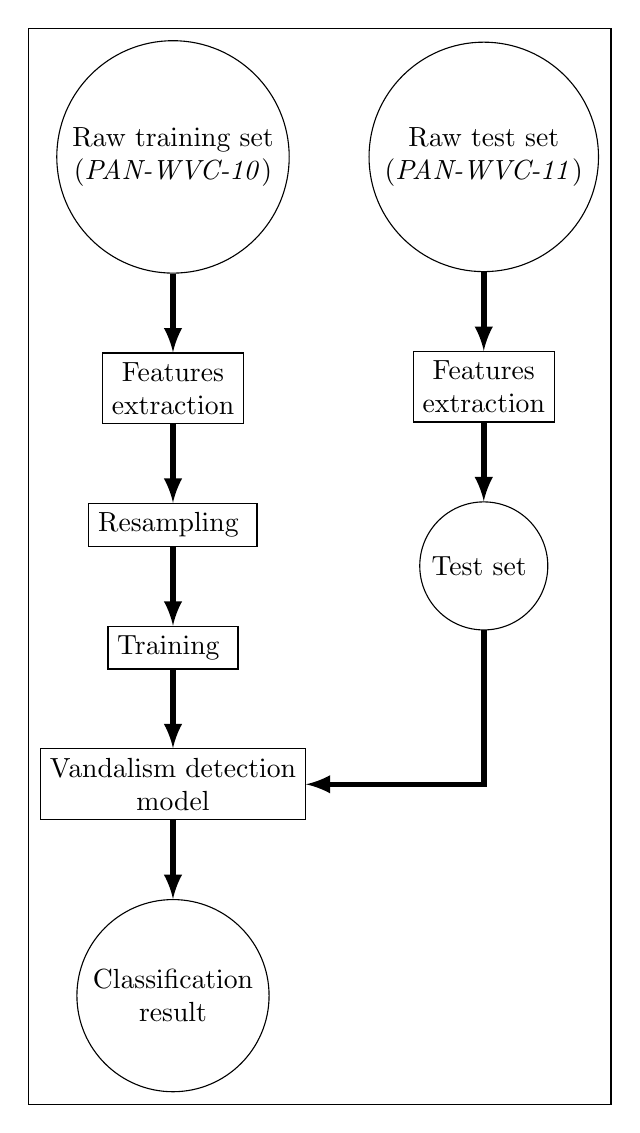
\begin{tikzpicture}[
	framed,
	nodes = {
		align = center
	},
	lines/.style={
		line width=2pt,
		>=latex
	},
	data/.style={
		circle,
		draw=black,
		text centered
	},
	proc/.style={
		rectangle,
		draw=black,
		text centered
	}
]
	\node[data] (training_raw) {
		Raw training set\\
		(\textit{PAN-WVC-10})
	};

	\node[proc] (wvcgen) [below=of training_raw] {
		Features\\
		extraction
	};

	\node[proc] (trainingset) [below=of wvcgen] {
		Resampling
	};

	\node[proc] (c)  [below=of trainingset] {
		Training
	};

	\node[proc] (m)  [below=of c] {
		Vandalism detection\\
		model
	};

	\node[data] (o)  [below=of m] {
		Classification\\
		result
	};
	%%
	\node[data] (testset_raw) [right=of training_raw] {
		Raw test set\\
		(\textit{PAN-WVC-11})
	};

	\node[proc] (testset_wvcgen) [below=of testset_raw] {
		Features\\
		extraction
	};

	\node[data] (testset) [below=of testset_wvcgen] {
		Test set
	};

	\draw[lines,->] (training_raw) -- (wvcgen);
	\draw[lines,->] (wvcgen) -- (trainingset);
	\draw[lines,->] (trainingset) -- (c);
	\draw[lines,->] (c) -- (m);
	\draw[lines,->] (m) -- (o);

	\draw[lines,->] (testset_raw) -- (testset_wvcgen);
	\draw[lines,->] (testset_wvcgen) -- (testset);

	\draw[lines,->] (testset) |- (m);
\end{tikzpicture}
}
\caption{
	Workflow process on detecting vandalism
}
\label{fig:proses}
\end{figure}


\subsection{Data Preparation}
	\label{subsection:data_preparation}
	The original dataset can not be used for training and testing, they need to
combined, cleaned by removing unneeded attributes, and cleaned on their revision
to generate features.

Dataset that is used for training is PAN-WVC-10 \cite{potthast2008automatic}.
which contain two separate set, the edit set and annotation set.
The two set then combined to get only their edit ID, class, old revision ID,
new revision ID, edit time, editor, article title, and edit comment.

Dataset for testing is an English dataset of PAN-WVC-11 \cite{potthast:2010b}.
The original attribute from the set is similar with PAN-WVC-10 except they were
already combined into single set.

PAN-WVC-10 and PAN-WVC-11 contain revision files.
Revision is history of edit that contain the current text in article based on
edit ID, where each ID in dataset reference to one revision file.

In both dataset, we then add two new attributes, deletions
(text that has been deleted in previous revision) and additions (text that
has been added in new revision).
Also, the class attribute value is replaced with numeric, where
"vandalism" become "1" and "regular" become "0".

The next step is to create revision text that is clean from wiki syntax, with
an aim to help in generating feature.
Every revision files cleaned up by removing URI, wiki markups, and wiki tokens.


\subsection{Extracting Features}
	Previous papers group the features into three categories which are metadata,
text, and language.
This paper use four metadata features, 11 text features, and 10
language features which has been used and analyzed in Mola-Velasco paper
\cite{mola2012wikipedia}.

All previous feature then implemented in a program.
The program then executed on PAN-WVC-10 and PAN-WVC-11 set that has been
prepared in section \ref{subsection:data_preparation}, which generate features
dataset contain continous values.
The implementation for combining, cleaning, and generating the features is
published as open source software as \texttt{wvcgen}
\footnote{\url{https://github.com/shuLhan/wvcgen}}.


\subsubsection{Metadata Features}
	Metadata feature references to the properties of revision which can be directly
taken, for example, identity of editor, comment, or the size of changes.
Below is list of metadata features,
\begin{itemize}
\item \textbf{Anonymous}. If the editor of revision is registered user then in
the edit set it contain their username.
\item \textbf{Comment length}. Counting number of character that left by editor
in comment field.
\item \textbf{Size increment}. An absolute size of new revision. Higher size
value can indicated as deletion on whole article.
\item \textbf{Size ratio}. The size of new revision divided by the size of old
revision.
\end{itemize}


\subsubsection{Text Features}
	Below is the list of text features that are used.

\begin{itemize}
\item \textbf{Ratio of lowercase and uppercase character}. The ratio is
computed in new revision by dividing number of uppercase characters with
lowercase characters.
\item \textbf{Ratio of uppercase to all characters}. Computed by dividing
number of uppercase characters with number of all characters in new revision.
\item \textbf{Digit ratio}. Computed by dividing number of digit with number of
all character in new revision.
\item \textbf{Ratio of non-alphanumeric characters}. Computed by dividing
number of all non-alphanumeric characters with number of all characters in new
revision.
\item \textbf{Character diversity}. Computed by counting number of unique
character divided by length of text in new revision.
\item \textbf{Character distribution}. Computed using Kullback-Leibler
divergence on old revision compared with text addition in new revision.
\item \textbf{Compression rate}. Computed by applying LZW compression algorithm
on inserted text.
\item \textbf{Good token}. Computed by counting number of token that vandal
rarely used on text, for example wiki syntax.
\item \textbf{Term frequencies}. Computed by counting number of unique words
added divided by number of unique words in new revision.
\item \textbf{Longest word}. Computed by counting number of character on the
longest word inserted.
\item \textbf{Length of similar character}. Computed by counting number of
similar characters used in sequence in single word, for example
\textit{aaarrrgghhhh}, \textit{sooo huge}.
\end{itemize}


\subsubsection{Language Features}
	Language features based on number of particular words that are inserted in new
revision.
For each word categories, there are two feature to be computed: frequency and
impact.
Frequency feature computed by counting number of words in category divided by
total number of words in new revision.
Impact feature computed by counting percentage of word usage in new revision
divided by total words in old and new revision.
Below is list of language features that are used.

\begin{itemize}
\item \textbf{Vulgarism}. Counting number of vulgar, harsh, and offensive
words.
\item \textbf{Subject}. Counting number of first or second person
words used in inserted text, including colloquial words, for example
\textit{I}, \textit{you}.
\item \textbf{Bias}. Counting number of bias words, for example "coolest",
"huge".
\item \textbf{Pornography}. Counting number of pornography related words
inserted in new revision.
\item \textbf{Bad words}. Counting number of bad, non-vulgar words, usually
indicated by bad writing. For example "wanna", "gotcha".
\item \textbf{All word categories}. Combination of all word categories.
\end{itemize}


\subsection{Resampling Dataset}
	PAN-WVC-10 without resample contain 2,394 positive or vandalism samples and
30,045 negative or regular samples.
The dataset then resampled using SMOTE and LNSMOTE for
positive class to get a balanced class.
For SMOTE, the parameter used for resampling is 1,200\% and parameter for
K-Nearest-Neighbour (KNN) is 5, which generate 28,728 synthetic samples, total of
positive sample combined with original sample result in 31,122 positive
samples.
Parameter for resampling using LNSMOTE is similar with SMOTE, which generate
28,588 positive synthetic samples, in total of 30,982 positive samples.
The implementation for SMOTE and LNSMOTE published as open source software
\footnote{\url{https://github.com/shuLhan/go-mining/tree/master/resampling}}.



\subsection{Classifier Implementations}

Implementation of classifiers carried out gradually.
Started by implementing Classification and Regression Trees (CART)
\cite{breiman1984classification}
which is used in Random Forest and Cascaded Random Forest.
The implementation of CART based on Jiawei Han et al. book, chapter 8
\cite{han2011data}.
The implementation of Random Forest is based on original paper of Breiman
\cite{breiman2001random}, plus additional resource from internet.
The implementation of Cascaded Random Forest is based on original paper of
Baumann et al.
\cite{baumann2013cascaded}.
The result of all implementation is published as open source software to help
others in future research or for real-world usage \footnote{\url{https://github.com/shuLhan/go-mining/tree/master/classifiers}}.


\subsection{Training and Testing}

There are three common parameter between RF and CRF which are 200 for number of
tree, 5 for number of random features, and 64\% for percentage of
bootstrapping.
For consistency, their value are constant between training.
For CRF classifier, three separated testing had been conducted using different
parameter for number of stage and number of tree which are 200 stages with 1
tree, 100 stages with 2 trees, and 50 stages with 4 trees; all of them have
equal total number of trees.
This is an experiment to see the effect of number of trees to stage and their
performance.
Another parameter for training with CRF are thresholds for true-positive rate
(TPR) and true-negative rate (TNR), which set to constant value 0.95 and 0.95
for all training.

\begin{table}[tp]
\caption{Dataset for training and testing.}
\centering
\begin{tabular}{|| c | l | c | c | c ||}
\hline
\multirow{2}{*}{Type} & \multirow{2}{*}{Resampling mode}
	& \multicolumn{3}{c||}{Number of sample} \\
\cline{3-5}
    & & Vandalism & Regular & Total \\
\hline
\hline
\multirow{3}{*}{Training} & -       &  2.394 & 30.045 & 32.439 \\
                              & SMOTE   & 27.728 & 30.045 & 58.773 \\
                              & LNSMOTE & 28.588 & 30.045 & 58.633 \\
\hline
Testing & - & 1.143 & 8.842 & 9.985 \\
\hline
\end{tabular}
\label{table:dataset}
\end{table}


The dataset used for training is PAN-WVC-10 which consist of three different
set, dataset without resampled, dataset resampled with SMOTE, and dataset
resampled with LNSMOTE.
The dataset used for testing is PAN-WVC-11 which contain 1,143 positive
samples and 8,842 negative samples, in total of 9985 samples.

Training is conducted by running each classifier program, RF and CRF, on
those three different PAN-WVC-10 feature dataset.
Testing is conducted after the model has been built by giving the model the
PAN-WVC-11 feature dataset as an input.

The environment used for training and testing is Intel\textregistered
Core\texttrademark i7-4750HQ CPU 2,00 GHz, with total 8 GB of RAM.
Each training is done separatedly to avoid cache miss which affect computation
time.


\section{Evaluation}
	\label{section:result_and_analysis}
	When detecting vandalism, it is better to receive false positive than missing
vandalism edit.
Wrong classification, when regular edit detected as vandalism, will give no
effect on reader, but missing on vandalism edit can lead to information loss,
fault information, or disturb the reader.
For this reason, our evaluation based on true-positive rate of classifier
performance.
True-positive rate (TPR) or recall is number of actual positive samples divided
by sum of sample positive classified as positive and sample positive classified
as negative (false-positive).
TPR has a value between 0 and 1, with value approaching to 0 indicate poor
performance and value approaching 1 indicate good performance.
Result of testing are given in terms of performance of each classifier on table
\ref{tab:stats} and training computation time on figure \ref{graph:runtimes}.

Result from CRF classifer on LNSMOTE with 200 stages and 1 tree have the
highest TPR value $0.9904$.
RF classifier without resampling gave the lowest TPR $0,1654$.

From the computation time, CRF classifier is faster than RF on all training.
Using RF and CRF with 50 stages and 4 trees as comparison, CRF without
resampling is 11 times faster than RF, and for dataset that has been resampled
with SMOTE and LNSMOTE, CRF is 1.6 times faster than RF.

	\DTLsetseparator{;}
\DTLloaddb{stats}{./stats.csv}
\DTLmaxforcolumn{stats}{TPR}{\maxtpr}
\DTLminforcolumn{stats}{FPR}{\minfpr}
\DTLmaxforcolumn{stats}{TNR}{\maxtnr}
\DTLmaxforcolumn{stats}{Presisi}{\maxprec}
\DTLmaxforcolumn{stats}{F-Measure}{\maxfm}
\DTLmaxforcolumn{stats}{Akurasi}{\maxacc}
\DTLmaxforcolumn{stats}{AUC}{\maxauc}

\begin{table}[tp]
\caption{Performance of Random Forest and Cascaded Random Forest}
\label{tab:stats}
\centering
\begin{tabular}{llrrrrrrr}
\hline
\textbf{Classifier} &
\textbf{Dataset} &
\textbf{TPR}
\DTLforeach*{stats}{%
	\cl=Klasifikasi,%
	\ds=Dataset,%
	\tpr=TPR%
}{%
	\DTLifnullorempty{\cl}
		{\\ \cline{2-3}}
		{\\ \hline}
	\DTLifnullorempty{\cl}
		{}
		{
			\multirow{3}{2cm}{\cl}
		}
	& \ds
	& \DTLifnumeq{\tpr}{\maxtpr}{\textbf{\tpr}}{\tpr}
}
\\
\hline
\end{tabular}
\end{table}


	\begin{figure}[htb]
\centering
\mytikzinput{graph_runtimes}
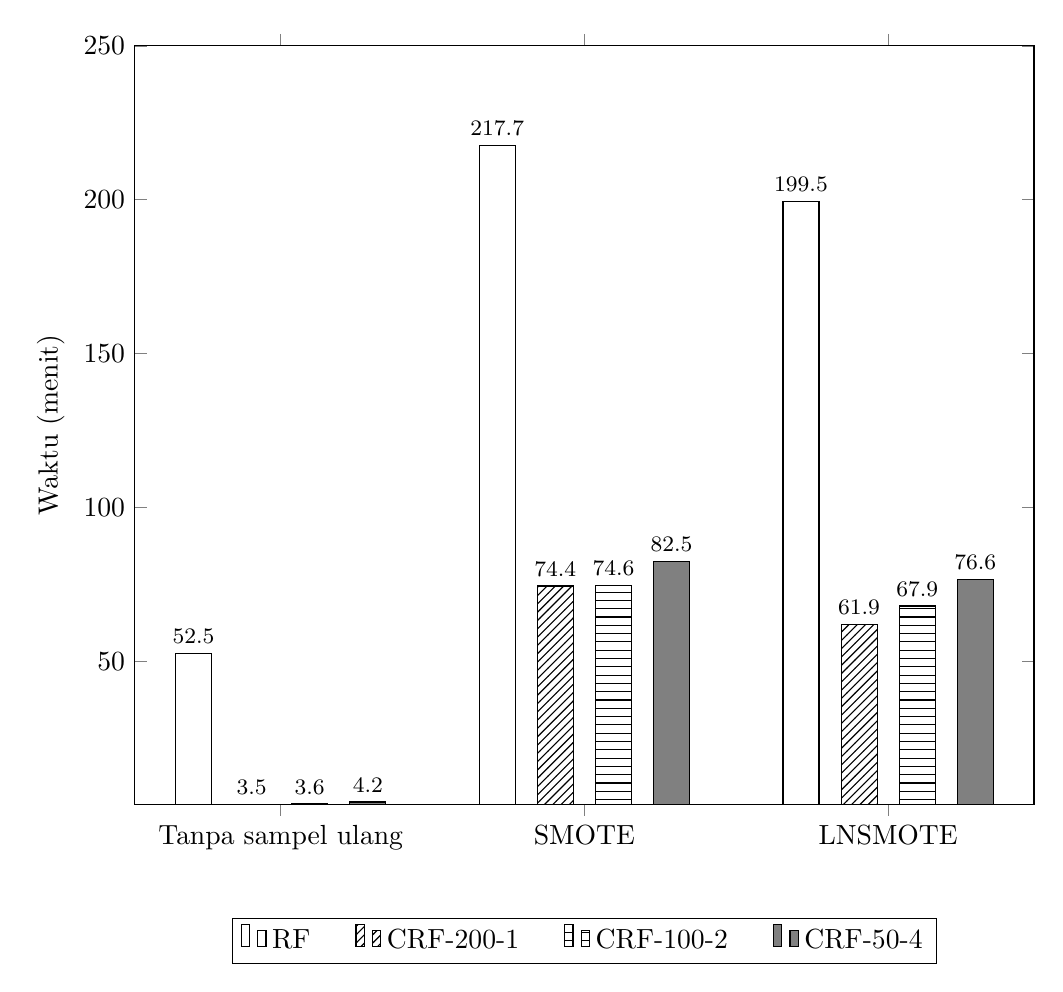
\begin{tikzpicture}
	\begin{axis}[
		width=13cm,
		ymax=250,
		ybar=8pt,
		ylabel=Waktu (menit),
		symbolic x coords={Tanpa sampel ulang, SMOTE, LNSMOTE},
		xtick=data,
		nodes near coords,
		every node near coord/.append style={font=\footnotesize},
		enlarge x limits=0.24,
		enlarge y limits=0,
		bar width = 13pt,
		legend style={
			at={(0.5,-0.15)},
			anchor=north,
			legend columns=-1,
			/tikz/every even column/.append style={column sep=0.5cm}
		},
	]
		%% RF
		\addplot[fill=white] coordinates {
			(Tanpa sampel ulang, 52.5)
			(SMOTE, 217.7)
			(LNSMOTE, 199.5)
		};

		%% CRF-200-1
		\addplot[pattern=north east lines] coordinates {
			(Tanpa sampel ulang, 3.5)
			(SMOTE, 74.4)
			(LNSMOTE, 61.9)
		};

		%% CRF-100-2
		\addplot[pattern=horizontal lines] coordinates {
			(Tanpa sampel ulang, 3.6)
			(SMOTE, 74.6)
			(LNSMOTE, 67.9)
		};

		%% CRF-50-4
		\addplot coordinates {
			(Tanpa sampel ulang, 4.2)
			(SMOTE, 82.5)
			(LNSMOTE, 76.6)
		};
	\legend{RF, CRF-200-1, CRF-100-2, CRF-50-4}
	\end{axis}
\end{tikzpicture}
\caption{Waktu pelatihan untuk setiap klasifikasi berdasarkan dataset.}
\label{graph:runtimes}
\end{figure}



\section{Conclusion}
\label{section:conclusion}

On average SMOTE increase TPR value by $0.19$ times while LNSMOTE, on average
increase TPR value $0.33$ times.
Another interisting effect of CRF classifier, when using less number of tree on
each stage on dataset without resampling, their performance almost similar with
CRF on resampling with more number of tree, for example performance of CRF with
100 stages and 2 trees on dataset without resampling is adjacent with CRF with
50 stages and 4 tress on dataset resampled with SMOTE.

The best classifier model for vandalism without resampling returned by CRF with
200 stages and 1 tree with TPR value $0.9668$.
The best classifier model for dataset that has been resampled with SMOTE is CRF
with 200 stages and 1 trees with TPR value $0.979$.
The best classifier model for dataset that has been resampled with LNSMOTE is
CRF with 200 stages and 1 trees with TPR value $0.9904$.
Overall, the best model is CRF with 200 stages and 1 trees on dataset resampled
with LNSMOTE.
From the computation time, CRF classifier is faster than RF on all training.
Using RF and CRF with 50 stages and 4 trees as comparison, CRF without
resampling is 11 times faster than RF, and for dataset that has been resampled
with SMOTE and LNSMOTE, CRF is 1.6 times faster than RF.

\section{Contribution}

This paper contribute on finding the best classifier on detecting vandalism on
Wikipedia and evaluating the effect of LNSMOTE resampling on imbalance dataset
and performance of CRF agains RF.
Apart from that, this paper also provides a framework to create and develop
vandalism features from raw PAN WVC dataset without having to build it again
from scratch.
Another contribution is a library for data processing and machine learning,
especially on resampling using LNSMOTE and CRF classifier which has no
open implementation on renowned program like Weka, Scikit-Learn, or R.
This framework can be used in the next research or in real-world application.

\section{Future Works}

All of training model on this paper were using RF and CRF algorithm in serial,
in which each tree is build one by one sequentially or when classifying sample
each of them was given as input to each tree sequentially to get their classes.
Using parallel algorithm, for building trees or classifying samples, can
speeding up training, testing and getting classifier result.
In the domain of machine learning, an interesting new algorithm is eXtreme
Gradient Boosting (XGBoost) \cite{chen2016xgboost}.
Using XGBoost on Wikipedia vandalism dataset maybe can increase the accuracy
of detection.

\bibliographystyle{IEEEtran}
\bibliography{IEEEabrv,bibliography}

\end{document}
